\documentclass[../main.tex]{subfiles}

% \title{Optical components}
% \date{2018-02-04}
% \author{Hongjie Lu}

\begin{document}

	% \maketitle
	% \pagenumbering{gobble}
	% \newpage
	\section{Refraction}
	\subsection{Planar interface}
	\begin{itemize}  
	\item Snell’s law
	\item external reflection $(n_1<n_2)$: ray refracted away from the interface
	\item internal reflection $(n_1>n_2)$: ray refracted towards the interface
	\item total internal reflection (TIR) for: $\theta_2 = \frac{\pi}{2}\Rightarrow sin\theta_1=sin\theta_{TIR}=\frac{n_2}{n_1}$
	Normally, the definitions of "internal" and "external" are with respect to the medium the light is emerged from. Total internal reflection is more common in application, however, total external reflection normally refers to X-rays whose indices of refraction for all materials are all slightly below 1. This entails that total reflection of X-rays only can occur when they travel through vacuum and impinge on a surface (at a small glancing angle). Since this kind of total reflection takes place outside of the material it is termed total external reflection.
	\end{itemize}
	\begin{figure}[h!]
	  \centering
	  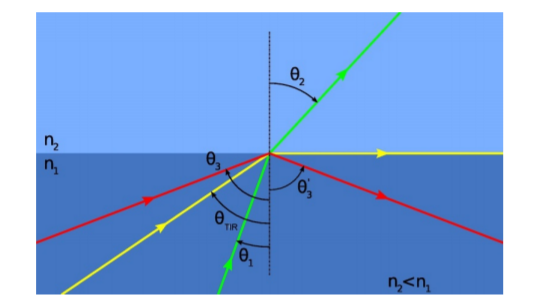
\includegraphics[scale=0.7]{../graphics/Optical_components6.png}
	  \caption{Planar interface}
	  \label{fig:interface1}
	\end{figure}
	\subsection{Spherical interface (paraxial)}
	as shown in "Geometrical optics" part
	\subsection{Spherical thin lens (paraxial)}
	as shown in "Geometrical optics" part

	\section{Reflection(Mirror)}
	\subsection{Planar mirror}
	\begin{itemize}  
	\item Rays originating from P1 are reflected and seem to originate from P2.
	\end{itemize}
	\begin{figure}[h!]
	  \centering
	  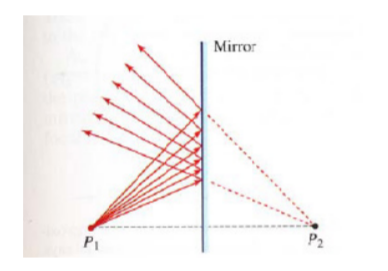
\includegraphics[scale=0.7]{../graphics/Optical_components1.png}
	  \caption{Planar mirror}
	  \label{fig:mirror1}
	\end{figure}

	\subsection{Paraboloidal mirror}
	\begin{itemize}  
	\item parabolic or paraboloid or paraboloidal mirror
	\item Parallel rays converge in the focal point (focal length f).
	\item Applications: Telescope, collimator
	\end{itemize}
	\begin{figure}[h!]
	  \centering
	  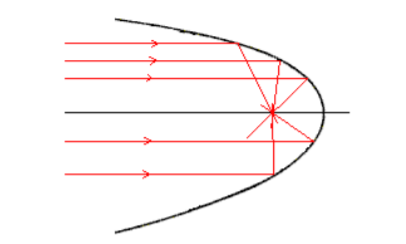
\includegraphics[scale=0.7]{../graphics/Optical_components2.png}
	  \caption{paraboloidal mirror}
	  \label{fig:mirror2}
	\end{figure}

	\subsection{Ellipsoidal mirror}
	\begin{itemize}  
	\item Rays originating from focal point $P_1$ converge in the second focal point $P_2$
	\end{itemize}
	\begin{figure}[h!]
	  \centering
	  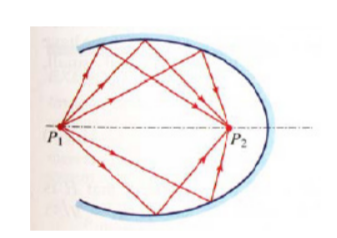
\includegraphics[scale=0.7]{../graphics/Optical_components3.png}
	  \caption{Ellipsoidal mirror}
	  \label{fig:mirror3}
	\end{figure}
	\FloatBarrier
	\subsection{Cylindrical mirror}
	%Kirkpatrick-Baez mirrors
	\subsection{Spherical mirror}
	\begin{figure}[h!]
	  \centering
	  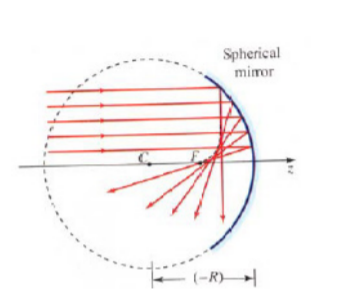
\includegraphics[scale=0.7]{../graphics/Optical_components4.png}
	  \caption{Spherical mirror}
	  \label{fig:mirror4}
	\end{figure}
	\begin{itemize}  
	\item Neither imaging like elliptical mirror nor focusing like parabolic mirror
	\item parallel rays cross the optical axis at different points
	\item connecting line of intersections of rays $\to$ caustic
	\item parallel, paraxial rays converge to the focal point $f = (-R)/2$
	\item convention: $R < 0$ - concave mirror; $R > 0$ - convex mirror
	\item for paraxial rays the spherical mirror acts as a focusing as well as an imaging optical element. paraxial rays emitted in point $P_1$ are reflected and converge in point $P_2$. $\frac{1}{z_1}+\frac{1}{z_2}\approx\frac{2}{-R}$
	\item paraxial imaging: imaging formula and magnification. $m=-\frac{z_2}{z_1}$
	\end{itemize}
	\begin{figure}[h!]
	  \centering
	  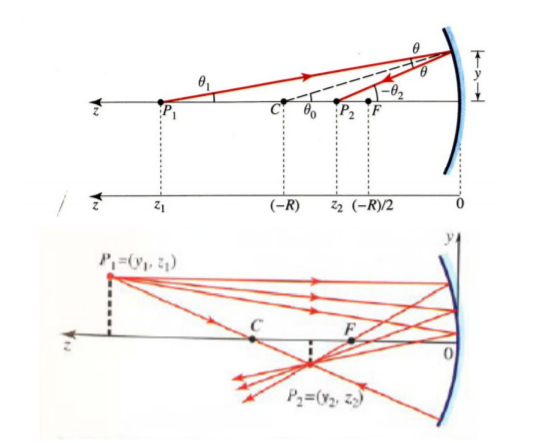
\includegraphics[scale=0.7]{../graphics/Optical_components5.png}
	  \caption{Spherical mirror paraxial}
	  \label{fig:mirror5}
	\end{figure}
	\FloatBarrier
	\subsection{Toroidal mirror}
	Toroidal mirrors are focusing devices having two different radii whose axes are oriented perpendicularly. They are utilized in instances where a beam must be focused and folded. Rather than using both a spherical mirror and a plane mirror for this purpose, both functions may be combined in one element. Toroidal mirrors also correct for the astigmatism that result when a spherical mirror is used off axis.\\
	Toroidal mirrors are aspherical mirrors where each curvature of orthogonal two axes (horizontal and vertical one) are different. Barrel or Tire shaped with a rotation axis are available.
	\begin{figure}[h!]
	  \centering
	  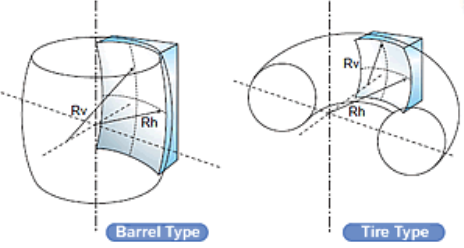
\includegraphics[scale=0.7]{../graphics/Optical_components7.png}
	  \caption{Toroidal mirror}
	  \label{fig:Toroidal}
	\end{figure}
	\section{reference}
	\href{http://www.iap.uni-jena.de/iapmedia/de/Lecture/Fundamentals+of+Modern+Optics1427752800/FoMO14_Script_2015_02_14s.pdf}{Lecture slide "Fundamentals of Modern Optics" of Jena}
	\section{Index}
	The Polar coordinates form of conic sections 
\end{document}